%!TEX root = practicum2.tex
% \todo[inline]{Bonus: Determine the fractal dimension of finite clusters as a function of $p$.}
\todo[inline]{Definitie van fractal dimension}

\todo[inline]{Welke fractal dimension hebben anderen gevonden?}

\todo[inline]{Boxcounting = Minkowski–Bouligand dimension uitleggen met source}
	\begin{equation}
		\text{dim}_{\text{box}} = \lim_{\epsilon \to 0} \frac{\log N(\epsilon)}{\log\left[ \frac{1}{\epsilon} \right]}.
	\end{equation}

We have used the function \t{boxcount} by \textcite{boxCounting} to determine the fractal dimension of different clusters. This method uses boxsizes that are power of two consequently $\varepsilon = 1, 2, 3, \dotsc 2^Q$ where $Q$ is the smallest integer such that $Q \leq (2N + 1)$. We have used the boxcounting algorithm on a cluster generated with $N= 80$, $p = 0.7$, the used cluster is shown in \cref{fig:exp_fractal:cluster}.

\begin{figure}
	\centering
	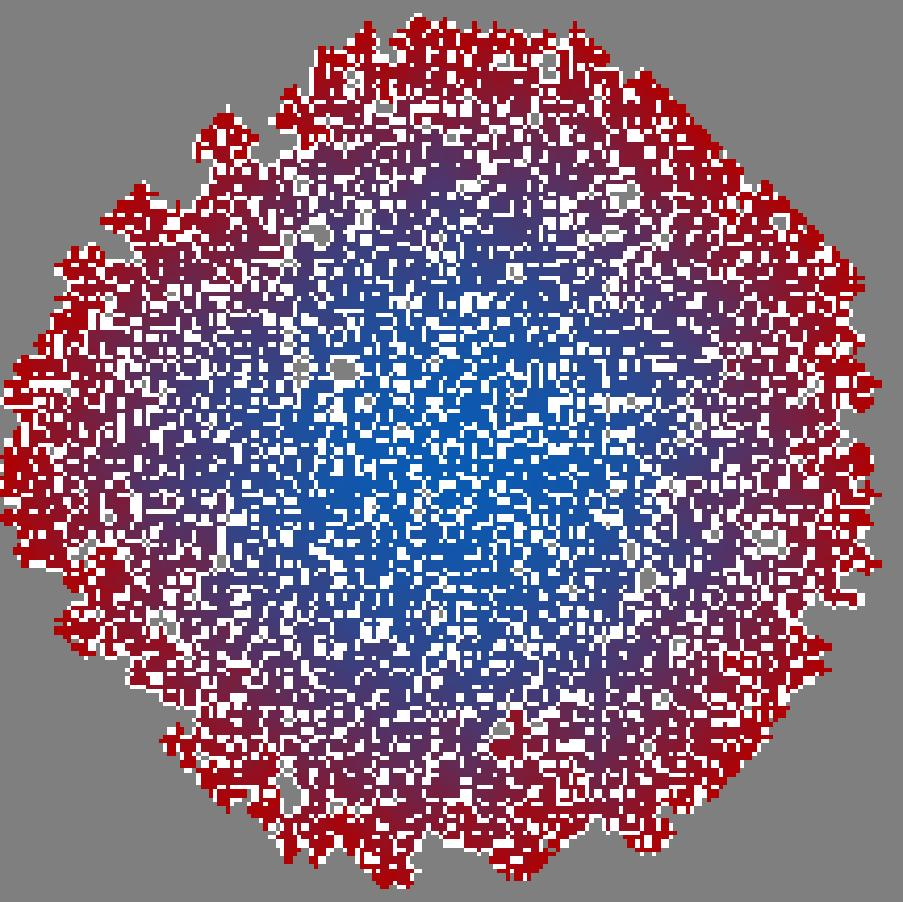
\includegraphics[width=1\columnwidth]{./img/assignment_fractal_cluster}
	\caption{The cluster used to determine the Minkowski-Bouligand dimension of clusters generated with percolation, the clusters was generated with $N = 80$, $p = 0.7$.}
	\label{fig:exp_fractal:cluster}
\end{figure}

\Cref{fig:exp_fractal:minkowskiDimension} presents the number of boxes as a function of the size of the boxes. \todo[inline]{Observatie}
\todo[inline]{Past de gevonden fractal dimension met de theorie?}

\begin{figure}
	\centering
	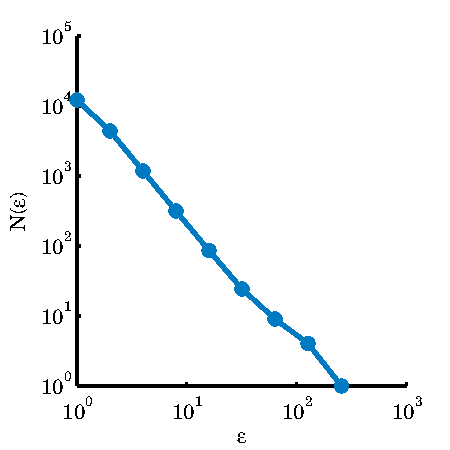
\includegraphics[width=1\columnwidth]{./img/assignment_fractal_numboxesVSboxsize}
	\caption{The number of boxes used to cover a cluster ($N = 80, p = 0.7$) as a function of the box size for the cluster presented in \cref{fig:exp_fractal:cluster}.}
	\label{fig:exp_fractal:minkowskiDimension}
\end{figure}


